\title{Assignment 5: CS 763, Computer Vision}
\author{Sasank Chilamkurthy\\ Tharun Kumar Reddy\\ Rajeev Puppala}

\date{Due 17th April before 11:55 pm (no late submissions will be allowed this time)}

\documentclass[11pt]{article}

\usepackage{amsmath}
\usepackage{cancel}
\usepackage{amssymb}
\usepackage{hyperref}
\usepackage{ulem,color}
\usepackage{graphicx}
\usepackage[margin=0.5in]{geometry}
\begin{document}
\maketitle


\begin{enumerate}
\item This question is inspired from one of the questions that was asked in class. We will prove why the value of the coherence between $m \times n$ measurement matrix $\mathbf{\Phi}$ (with all rows normalized to unit magnitude) and $n \times n$ orthonormal representation matrix $\mathbf{\Psi}$ must lie within the range $(1,\sqrt{n})$. Recall that the coherence is given by the formula
$\mu(\mathbf{\Phi},\mathbf{\Psi}) = \sqrt{n} \textrm{max}_{i,j \in \{0,1,...,n-1\}} |\mathbf{\Phi^i}^t \mathbf{\Psi_j}|$. 
Proving the upper bound should be very easy for you. To prove the lower bound, proceed as follows. Consider a unit vector $\mathbf{g} \in \mathbb{R}^n$. We know that it can be expressed as $\mathbf{g} = \sum_{k=1}^n \alpha_k \mathbf{\Psi_k}$ as $\mathbf{\Psi}$ is an orthonormal \emph{basis}. Now prove that $\mu(\mathbf{\Psi},\mathbf{g}) = \textrm{max}_{i \in \{0,1,...,n-1\}} \dfrac{|\alpha_i|}{\sum_{j=1}^n \alpha^2_j}$. Exploiting the fact that $\mathbf{g}$ is a unit vector, prove that the minimal value of coherence is given by $\mathbf{g} = \sqrt{1/n} \sum_{k=1}^n \mathbf{\Psi_k}$ and hence the minimal value of coherence is 1. \textsf{[3 points]}\\
Sol. Coherence is given by $\mu(\mathbf{\Phi},\mathbf{\Psi}) = \sqrt{n} \textrm{max}_{i,j \in \{0,1,...,n-1\}} |\mathbf{\Phi^i}^t \mathbf{\Psi_j}|$.\\
$\mathbf{\Phi}$ has all rows normalized to unit magnitude and $\mathbf{\Psi}$ is an orthonormal matrix. so \\
$\textrm{max}_{i,j \in \{0,1,...,n-1\}} |\mathbf{\Phi^i}^t \mathbf{\Psi_j}|$ is $1$ therefore upperbound is $\sqrt{n}$.\\
$\|\mathbf{\Phi^i}\|^2 = \sum_{j \geq 1}|\phi^i\psi_j|^2 = 1$\\
$\implies \textrm{max}_{j \in \{0,1,...,n-1\}}|\phi^i\psi_j|^2 \geq \frac{1}{n}$ (As atleast one term should be greater than $\frac{1}{\sqrt{n}})$\\
$\implies|\phi^i\psi_j| \geq \frac{1}{\sqrt{n}}$\\
Therefore the lower bound of Coherence is 1.

\item A very beautiful aspect of compressive sensing is the rigorous mathematical basis - in the form of concrete error bounds on reconstruction results. While using regularization to solve ill-posed problems is a known technique in computer vision and image processing, the existence of error bounds is a unique feature for compressive sensing problems. What is more, the proof of these stunning results is actually not super-hard, and any (motivated) graduate or undergraduate student with a basic knowledge of properties of vectors, and (more than) a little bit of patience, can easily follow the proofs. The purpose of this exercise is to take you through the proof of the following theorem proved by Emmanuel Candes: \textsf{[12 points]}
\\
\textbf{Theorem:} Let $\mathbf{y} = \mathbf{Ax}+\mathbf{\eta}$ be a vector of noisy compressed measurements where the matrix $\mathbf{A} \in \mathbb{R}^{m \times n},  m \ll n$ has restricted isometry constant $\delta_{2s} < \sqrt{2}-1$. Let the noise magnitude be upper bounded as $\|\mathbf{\eta}\|_2 \leq \epsilon$. Let $\mathbf{x}^{\star}$ be the solution to the problem $\textrm{min}_{\mathbf{x}} \|\mathbf{x}\|_1$ such that $\|\mathbf{y} - \mathbf{Af}\|_2 \leq \epsilon$. Then $\mathbf{x^{\star}}$ obeys 
$\|\mathbf{x^{\star} - x}\|_2 \leq C_0 s^{-1/2}\|\mathbf{x - x_s}\|_1  + C_1 \epsilon$ where $C_0$ and $C_1$ are small-valued constants and $\mathbf{x_s}$ is a vector obtained by nullifying all entries of $\mathbf{x}$ except the $s$ entries with the largest absolute value. 
\\
\\
The proof is given below. Your job is to trace through it, verifying every step, and then answering the questions presented in blue colored font. \emph{Ideally, edit the latex file itself and write your answer in blue colored font}.
You will need to use the triangle inequality ($\|\mathbf{x}\|_2 + \|\mathbf{y}\|_2 \geq \|\mathbf{x}+\mathbf{y}\|_2$), the reverse triangle inequality ($\|\mathbf{x}-\mathbf{y}\|_2 \geq \|\mathbf{x}\|_2 - \|\mathbf{y}\|_2$), the Cauchy-Schwartz inequality (the dot product $|\langle \mathbf{x}, \mathbf{y} \rangle| \leq \|\mathbf{x}\|_2 \|\mathbf{y}\|_2$) for vectors $\mathbf{x}$ and $\mathbf{y}$, and the restricted isometry property for $\mathbf{A}$. Also remember that $\|\mathbf{x}\|_1 = \sum_i |x_i|$, $\|\mathbf{x}\|_2 = \sqrt{\sum_i x^2_i}$ and $\|\mathbf{x}\|_{\infty} = \textrm{max}_i |x_i|$.
\\
\\
\textbf{Proof:}
\\
\begin{enumerate}
\item We can write the following result: $\|\mathbf{A(x-x^{\star})}\|_2 \leq 2\epsilon$. \textcolor{blue}{(How is this derived?)}\\
\textcolor{blue}{$\|\mathbf{A(x-x^{\star})}\|_2 = \|\mathbf{Ax-Ax^{\star}}\|_2$\\
$\implies \|\mathbf{A(x-x^{\star})}\|_2 = \|\mathbf{y-Ax^{\star}-n}\|_2$\\
$\implies \|\mathbf{A(x-x^{\star})}\|_2 \leq \|\mathbf{y-Ax^{\star}}\|_2 + \|\mathbf{n}\|_2$ (triangle inequality)\\
$\implies \|\mathbf{A(x-x^{\star})}\|_2 \leq \epsilon + \epsilon$\\
$\implies \|\mathbf{A(x-x^{\star})}\|_2 \leq 2\epsilon$}
\item Let us define vector $\mathbf{h} = \mathbf{x^{\star}-x}$. Let us denote vector $\mathbf{h_T}$ as the vector equal to $\mathbf{h}$ only on an index set $T$ and zero at all other indices. Let $T_0$ the set of indices containing the $s$ largest entries of $\mathbf{x}$ (in terms of absolute value), $T_1$ be the set of indices of the next $s$ largest entries of $\mathbf{x}$, $T_2$ be the set of indices of the next $s$ largest entries of $\mathbf{x}$ after $T_1$, and so on. We will now decompose $\mathbf{h}$ as the sum of $\mathbf{h_{T_0}}, \mathbf{h_{T_1}}, \mathbf{h_{T_2}}, ...$. We will denote the complement of an index set $T$ as $T^c$. Our aim will be to prove that both $\|\mathbf{h_{T_0 \cup T_1}}\|_2$ and $\|\mathbf{h_{(T_0 \cup T_1)^c}}\|_2$ are upper bounded by sensible and intuitive quantities. 
\item We will first prove the bound on $\|\mathbf{h}_{(T_0 \cup T_1)^c}\|_2$, in the following way, using simple vector properties and the fact that $\mathbf{x+h}$ is the minimum of the objective function subject to the given constraint. 
\begin{enumerate}
\item We have $\|\mathbf{h}_{T_j}\|_2 \leq s^{1/2} \|\mathbf{h}_{T_j}\|_\infty \leq s^{-1/2} \|\mathbf{h}_{T_{j-1}}\|_1$. \textcolor{blue}{(Prove both these inequalities. Note that any element of $T_{j-1}$ is greater than or equal to any element of $T_j$ for any $j \geq 1$)}.\\
\textcolor{blue}{$\|\mathbf{h}_{T_j}\|_2 \leq \sqrt{s\textrm{max}_i |x_i|^2} $ \\
$\implies \|\mathbf{h}_{T_j}\|_2 \leq s^\frac{1}{2}\textrm{max}_i |x_i|$\\
$\implies \|\mathbf{h}_{T_j}\|_2 \leq s^\frac{1}{2}\|\mathbf{h}_{T_j}\|_\infty$\\
Any element of $T_{j-1}$ is greater than or equal to any element of $T_j$\\
$\therefore \|\mathbf{h}_{T_j}\|_\infty \leq$ least element of $T_{j-1} \leq \frac{\|\mathbf{h}_{T_{j-1}}\|_1}{s}$\\
$\implies s^\frac{1}{2}\|\mathbf{h}_{T_j}\|_\infty \leq s^\frac{-1}{2}\|\mathbf{h}_{T_{j-1}}\|_1$}
\item Therefore $\sum_{j \geq 2}\|\mathbf{h}_{T_j}\|_2 \leq s^{-1/2} \|\mathbf{h}_{(T_0)^c}\|_1$. \textcolor{blue}{(Prove this inequality)}.\\ 
\textcolor{blue}{$\sum_{j \geq 2}\|\mathbf{h}_{T_j}\|_2 \leq s^\frac{-1}{2}\sum_{j \geq 2}\|\mathbf{h}_{T_{j-1}}\|_1$\\
$\implies \sum_{j \geq 2}\|\mathbf{h}_{T_j}\|_2 \leq s^\frac{-1}{2}\sum_{k \geq 2}\|\mathbf{h}_{T_k}\|_1$\\
$\implies \sum_{j \geq 2}\|\mathbf{h}_{T_j}\|_2 \leq s^{-1/2} \|\mathbf{h}_{(T_0)^c}\|_1$}
\item Hence we have $\|\mathbf{h}_{(T_0 \cup T_1)^c}\|_2 = \|\sum_{j \geq 2} \mathbf{h}_{T_j}\|_2 \leq \sum_{j \geq 2} \|\mathbf{h}_{T_j}\|_2 \leq s^{-1/2} \|\mathbf{h}_{(T_0)^c}\|_1$ (\textcolor{blue}{Prove both inequalities}).\\
\textcolor{blue}{$\|\mathbf{h}_{(T_0 \cup T_1)^c}\|_2 = \|\sum_{j \geq 2} \mathbf{h}_{T_j}\|_2$\\
$\|\sum_{j \geq 2} \mathbf{h}_{T_j}\|_2 \leq \sum_{j \geq 2} \|\mathbf{h}_{T_j}\|_2$ ( From Triangle Inequality)\\
Above result shows that$\sum_{j \geq 2} \|\mathbf{h}_{T_j}\|_2 \leq s^{-1/2} \|\mathbf{h}_{(T_0)^c}\|_1$\\
$\implies \|\mathbf{h}_{(T_0 \cup T_1)^c}\|_2 \leq s^{-1/2} \|\mathbf{h}_{(T_0)^c}\|_1$}
\item Now it turns out that $\|\mathbf{h}_{(T_0)^c}\|_1$ is not very large in value. Why so? As $\mathbf{x}^{\star}$ is the minimum, we have $\|\mathbf{x}\|_1 \geq \|\mathbf{x}+\mathbf{h}\|_1 = \sum_{i \in T_0} |x_i + h_i| + \sum_{i \in {(T_0)}^c} |x_i + h_i| \geq \|\mathbf{x}_{T_0}\|_1 - \|\mathbf{h}_{T_0}\|_1 + \|\mathbf{h}_{{(T_0)}^c}\|_1 - \|\mathbf{x}_{{(T_0)^c}}\|_1$ \textcolor{blue}{Prove the last inequality}. \\
\textcolor{blue}{$\sum_{i \in T_0} |x_i + h_i| + \sum_{i \in {(T_0)}^c} |x_i + h_i| = \sum_{i \in T_0} |x_i - (-h_i)| + \sum_{i \in {(T_0)}^c} |x_i -(- h_i)|$\\
$\implies \sum_{i \in T_0} |x_i + h_i| + \sum_{i \in {(T_0)}^c} |x_i + h_i| \geq \sum_{i \in T_0} |x_i| - \sum_{i \in T_0}|h_i| + \sum_{i \in {(T_0)}^c} |x_i| - \sum_{i \in T_0}|h_i|$ (Reverse Triangle Inequality)\\
$\implies \sum_{i \in T_0} |x_i + h_i| + \sum_{i \in {(T_0)}^c} |x_i + h_i| \geq \|\mathbf{x}_{T_0}\|_1 - \|\mathbf{h}_{T_0}\|_1 + \|\mathbf{h}_{{(T_0)}^c}\|_1 - \|\mathbf{x}_{{(T_0)^c}}\|_1$}
\item Rearranging the terms now gives us $\|\mathbf{h}_{{(T_0)}^c}\|_1 \leq \|\mathbf{h}_{{(T_0)}}\|_1  + 2\|\mathbf{x}_{{(T_0)^c}}\|_1 = \|\mathbf{h}_{{(T_0)}}\|_1  + 2\|\mathbf{x}-\mathbf{x_s}\|_1$. 
\item Combining everything, we now have $\|\mathbf{h}_{(T_0 \cup T_1)^c}\|_2 \leq s^{-1/2}(\|\mathbf{h}_{{(T_0)}}\|_1  + 2\|\mathbf{x}-\mathbf{x_s}\|_1) \leq \|\mathbf{h}_{{(T_0)}}\|_2 + \textcolor{red}{2}s^{-1/2} \|\mathbf{x}-\mathbf{x_s}\|_1$. \textcolor{blue}{(Prove the last inequality).}\\
\textcolor{blue}{From result in $(iii)$ we have $\|\mathbf{h}_{(T_0 \cup T_1)^c}\|_2 \leq s^{-1/2}\|\mathbf{h}_{(T_0)^c}\|_1$\\
Now using the result in $(iv)$ we get $\|\mathbf{h}_{(T_0 \cup T_1)^c}\|_2 \leq s^\frac{-1}{2}\|\mathbf{h}_{{(T_0)}}\|_1 + 2s^{-1/2} \|\mathbf{x}-\mathbf{x_s}\|_1 $\\
$s^\frac{-1}{2}\|\mathbf{h}_{{(T_0)}}\|_1 \leq \|\mathbf{h}_{{(T_0)}}\|_2$ (AM-QM inequality)\\
$\implies \|\mathbf{h}_{(T_0 \cup T_1)^c}\|_2 \leq \|\mathbf{h}_{{(T_0)}}\|_2 + 2s^{-1/2} \|\mathbf{x}-\mathbf{x_s}\|_1$}
\end{enumerate}
\item We will now prove the bound on $\|\mathbf{h}_{(T_0 \cup T_1)}\|_2$, in the following way. 
\begin{enumerate}
\item We observe that $\mathbf{Ah_{T_0 \cup T_1}} = \mathbf{Ah} - \sum_{j \geq 2} \mathbf{Ah_{T_j}}$. \\
Hence $\|\mathbf{Ah_{T_0 \cup T_1}}\|^2_2 = \langle \mathbf{Ah_{T_0 \cup T_1}} , \mathbf{Ah}\rangle - \langle \mathbf{Ah_{T_0 \cup T_1}} , \sum_{j \geq 2} \mathbf{Ah_{T_j}}\rangle$.
\item Now, we have $|\langle \mathbf{Ah}_{T_0 \cup T_1} , \mathbf{Ah}\rangle| \leq \|\mathbf{Ah}_{T_0 \cup T_1}\|_2 \|\mathbf{Ah}\|_2 \leq 2 \epsilon \sqrt{1 + \textcolor{red}{\cancel{2}}\delta_{2s}} \|\mathbf{h}_{T_0 \cup T_1}\|_2$ \textcolor{blue}{(Prove both these inequalities, one of which uses the restricted isometry property of $\mathbf{A}$)}.\\
\textcolor{blue}{$|\langle \mathbf{Ah}_{T_0 \cup T_1} , \mathbf{Ah}\rangle| \leq \|\mathbf{Ah}_{T_0 \cup T_1}\|_2 \|\mathbf{Ah}\|_2$ (Cauchy-Schwartz Inequality)\\
From the restricted isometry property of $\mathbf{A}$ we get\\
 $ \|\mathbf{Ah}_{T_0 \cup T_1}\|_2 \leq \sqrt{1 + \delta_{2s}} \|\mathbf{h}_{T_0 \cup T_1}\|_2$\\
 From the result in $(a)$ we have\\
 $ \|\mathbf{Ah}\|_2 \leq 2\epsilon$\\
 $\therefore |\langle \mathbf{Ah}_{T_0 \cup T_1} , \mathbf{Ah}\rangle| \leq \|\mathbf{Ah}_{T_0 \cup T_1}\|_2 \|\mathbf{Ah}\|_2 \leq 2 \epsilon \sqrt{1 + \delta_{2s}} \|\mathbf{h}_{T_0 \cup T_1}\|_2$}
\item We also have $|\langle \mathbf{Ah}_{T_0}, \mathbf{Ah}_{T_j}\rangle| \leq \delta_{2s} \|\mathbf{h}_{T_0}\|_2 \|\mathbf{h}_{T_j}\|_2$. To prove this, observe that $\mathbf{h_{T_0}}$ and $\mathbf{h_{T_j}}$ are vectors with disjoint support. $|\langle \mathbf{Ah}_{T_0}, \mathbf{Ah}_{T_j}\rangle| = \|\mathbf{h}_{T_0}\|_2 \|\mathbf{h}_{T_j}\|_2|\langle \mathbf{A\hat{h}}_{T_0}, \mathbf{A\hat{h}}_{T_j}\rangle|$  where $\mathbf{\hat{h}_{T_0}}$ and $\mathbf{\hat{h}_{T_j}}$ are unit-normalized vectors. This further yields $|\langle \mathbf{Ah}_{T_0}, \mathbf{Ah}_{T_j}\rangle|=\|\mathbf{h}_{T_0}\|_2 \|\mathbf{h}_{T_j}\|_2 \frac{\|\mathbf{A}(\mathbf{\hat{h}_{T_0}}+\mathbf{\hat{h}_{T_j}})\|^2 - \|\mathbf{A}(\mathbf{\hat{h}_{T_0}}-\mathbf{\hat{h}_{T_j}})\|^2}{4} 
\\ \leq \|\mathbf{h}_{T_0}\|_2 \|\mathbf{h}_{T_j}\|_2 \frac{(1+\delta_{2s})(\|\mathbf{h_{T_0}}\|^2+\|\mathbf{h_{T_j}}\|^2)-(1-\delta_{2s})(\|\mathbf{h_{T_0}}\|^2+\|\mathbf{h_{T_j}}\|^2)}{4} \\
= \delta_{2s} \|\mathbf{h}_{T_0}\|_2 \|\mathbf{h}_{T_j}\|_2$. Analogously, $|\langle \mathbf{Ah}_{T_1}, \mathbf{Ah}_{T_j}\rangle| \leq \delta_{2s} \|\mathbf{h}_{T_1}\|_2 \|\mathbf{h}_{T_j}\|_2$. 
\item Now, we have $(1-\delta_{2s})\|\mathbf{h}_{T_0 \cup T_1}\|^2_2 
\leq \|\mathbf{Ah}_{T_0 \cup T_1}\|^2_2 \leq 2 \epsilon \sqrt{1+\delta_{2s}}\|\mathbf{h}_{T_0 \cup T_1}\|_2 + \delta_{2s}(\|\mathbf{h}_{T_0}\|_2 + \|\mathbf{h}_{T_1}\|_2) \sum_{j \geq 2} \|\mathbf{h}_{T_j}\|_2$. \textcolor{blue}{(Prove this).} \\
\textcolor{blue}{From result in $d(i)$ we have\\
$\|\mathbf{Ah_{T_0 \cup T_1}}\|^2_2 = \langle \mathbf{Ah_{T_0 \cup T_1}} , \mathbf{Ah}\rangle - \langle \mathbf{Ah_{T_0 \cup T_1}} , \sum_{j \geq 2} \mathbf{Ah_{T_j}}\rangle$\\
From $d(ii)$ we have\\ 
$|\langle \mathbf{Ah}_{T_0 \cup T_1} , \mathbf{Ah}\rangle| \leq 2 \epsilon \sqrt{1 + \delta_{2s}} \|\mathbf{h}_{T_0 \cup T_1}\|_2$\\
From $d(iii)$ we have \\
$|\langle \mathbf{Ah}_{T_1}, \mathbf{Ah}_{T_j}\rangle| \leq \delta_{2s} \|\mathbf{h}_{T_1}\|_2 \|\mathbf{h}_{T_j}\|_2$\\
$\implies \langle \mathbf{Ah_{T_0 \cup T_1}} , \sum_{j \geq 2} \mathbf{Ah_{T_j}}\rangle \leq \delta_{2s}\|\mathbf{h_{T_0 \cup T_1}}\|_2\|\sum_{j \geq 2}\mathbf{h_{T_j}}\|_2 \leq \delta_{2s}\|\mathbf{h_{T_0 \cup T_1}}\|_2\sum_{j \geq 2}\|\mathbf{h_{T_j}}\|_2$\\
$\implies \|\mathbf{Ah}_{T_0 \cup T_1}\|^2_2 \leq 2 \epsilon \sqrt{1+\delta_{2s}}\|\mathbf{h}_{T_0 \cup T_1}\|_2 + \delta_{2s}(\|\mathbf{h}_{T_0}\|_2 + \|\mathbf{h}_{T_1}\|_2) \sum_{j \geq 2} \|\mathbf{h}_{T_j}\|_2$}
Furthermore, we can write $(1-\delta_{2s})\|\mathbf{h}_{T_0 \cup T_1}\|^2_2  \leq \|\mathbf{h}_{T_0 \cup T_1}\|_2(2\epsilon\sqrt{1+2\delta_{2s}}) + \sqrt{2}\delta_{2s} \sum_{j \geq 2} \|\mathbf{h}_{T_j}\|_2)$ because $\mathbf{h}_{T_0}$ and $\mathbf{h}_{T_1}$ are vectors with disjoint sets of non-zero indices and hence $\|\mathbf{h}_{T_0}\|_2 + \|\mathbf{h}_{T_1}\|_2 \leq \sqrt{2} \|\mathbf{h}_{T_0 \cup T_1}\|_2$.
\item Rearranging the above equation, and using one of the previous results (\textcolor{blue}{which one?}), 
we get $\|\mathbf{h}_{T_0 \cup T_1}\|_2 \leq \epsilon \dfrac{2\sqrt{1+\delta_{2s}}}{1-\delta_{2s}} + \dfrac{\sqrt{2}\sqrt{\delta_{2s}}}{1-\delta_{2s}} s^{-1/2} \|\mathbf{h}_{(T_0)^c}\|_1 
\\ \leq \epsilon \dfrac{2\sqrt{1+\delta_{2s}}}{1-\delta_{2s}} + \dfrac{\sqrt{2}\textcolor{red}{\cancel{\sqrt{\delta_{2s}}}} \textcolor{red}{\delta_{2s}}}{1-\delta_{2s}} \|\mathbf{h}_{T_0 \cup T_1}\|_2 + \dfrac{\sqrt{2}\delta_{2s}\textcolor{red}{\cancel{\sqrt{\delta_{2s}}}}}{1-\delta_{2s}} s^{-1/2} \|\mathbf{x}-\mathbf{x_s}\|_1$. Further rearranging gives us
$\|\mathbf{h}_{T_0 \cup T_1}\|_2  \leq C' \epsilon + C'' s^{-1/2} \|\mathbf{x}-\mathbf{x_s}\|_1$ where $C'$ and $C''$ are constants that depend only on $\delta_{2s}$ (note in particular that they do not depend on $n$).
\end{enumerate}
\item Now, we combine the upper bounds on $\|\mathbf{h}_{(T_0 \cup T_1)}\|_2$ and $\|\mathbf{h}_{(T_0 \cup T_1)^c}\|_2$ to yield the final result as follows: \\
$\|\mathbf{h}\|_2 \leq \|\mathbf{h}_{T_0 \cup T_1}\|_2 + \|\mathbf{h}_{(T_0 \cup T_1)^c}\|_2 \leq \|\mathbf{h}_{T_0 \cup T_1}\|_2 + \|h_{T_0}\|_2 + 2s^{-1/2}\|\mathbf{x}-\mathbf{x_s}\|_1 \\
\leq 2 \|\mathbf{h}_{T_0 \cup T_1}\|_2 + 2\textcolor{red}{s^{-1/2}}\|\mathbf{x}-\mathbf{x_s}\|_1 \leq C_0 s^{-1/2} \|\mathbf{x}-\mathbf{x_s}\|_1 + C_1 \epsilon$ \textcolor{blue}{(Justify all these inequalities. Write the final expression for $C_0$ and $C_1$ and explain where the sufficient condition $\delta_{2s} \leq \sqrt{2}-1$ arises)}.\\
\textcolor{blue}{Here first inequality comes from Triangle Inequality\\
Second inequality comes from $c(vi)$\\
Third inequality comes from fact that $\|h_{T_0}\|_2 \leq \|\mathbf{h}_{T_0 \cup T_1}\|_2 $\\
Fourth Inequality comes from $e(v)$\\
Comparison gives $C_1 = \frac{\epsilon4\sqrt{1+\delta_{2s}}}{1-(\sqrt{2}+1)\delta_{2s}}$ and $C_0 = 2+\frac{2\sqrt{2}\delta_{2s}}{1-(\sqrt{2}+1)\delta_{2s}}$\\
Here $C_1$ cant be negative so $1-(\sqrt{2}+1)\delta_{2s} \geq 0$\\
$\implies \delta_{2s} \leq \sqrt{2}-1$}
\end{enumerate}

\item In this section, you will implement the orthogonal matching pursuit (OMP) algorithm for reconstruction from compressive measurements. For this, first extract all overlapping patches of size $8 \times 8$ from the barbara image in the homework folder. Generate a $n \times n$ matrix $\mathbf{\Phi}$ where $n = 64$ with all entries sampled from a zero-mean Gaussian distribution of unit standard deviation. Let $\mathbf{\Phi}_m$ denote a submatrix consisting of the first $m$ ($m \leq n$) rows of $\mathbf{\Phi}$. 
\\
\\
Generate compressive measurements for each patch in the form $\mathbf{y_i} = \mathbf{\Phi}_m \mathbf{x_i}$ where $i$ is a patch index. Add zero mean Gaussian noise with standard deviation = 0.05 times the mean absolute value of all elements from the (non-noisy) coded patches. Your job is to recover $\mathbf{x_i}$ given $\mathbf{y_i}$ and $\mathbf{\Phi}_m$ for all $i$ using OMP. Since image patches are not sparse in the spatial domain, but sparse (or compressible) in the DCT domain, we will represent each patch as $\mathbf{x_i} = \mathbf{U \theta_i}$ where $\mathbf{U}$ is the 2D DCT matrix , and recover $\mathbf{\theta_i}$ first, thereafter reconstructing $\mathbf{x_i} = \mathbf{U} \mathbf{\theta_i}$. The final image should be reconstructed by averaging the overlapping patches in a sliding window fashion. 
\\
\\
You should repeat this experiment for $m = \textrm{ceiling}(fn)$ where $f \in \{0.9,0.8,0.7,0.6,0.5,0.4,0.3,0.2,0.1,0.05\}$ and record the mean squared patch error (MSPE) and mean squared image error (MSIE) each time. MSPE is given as the average of the mean squared error between the original and reconstructed patches. MSIE is the mean squared error between the original and reconstructed image. Plot a graph of both errors w.r.t. $m$. 
\\
\\
Repeat this experiment but using pseudo-inverse (the backslash operator in MATLAB) instead of OMP and plot the same errors. Comment on your observations.
\\
\\
Now, repeat the same experiment using OMP, but this time generating compressed measurements using the matrix $\mathbf{\Phi}_m$ which consists of a randomly generated subset of $m$ rows of the 2D DCT matrix $\mathbf{U}^T$. Again plot the errors. Comment on your observations. \textsf{[15 points]}.
\\
\\
(Important tip: Generate the 2D DCT matrix in MATLAB as follows: $U = kron(dctmtx(8)',dctmtx(8)')$ and \emph{not} as $U = dctmtx(64)'$. This is because the latter generates a 1D DCT matrix, and images are not sparse in that basis.)
\begin{itemize}
\item[Ans.] Complete images and reports are available in html folder as hw5.html, hw5\_2.html and hw5\_3.html. As can be expected errors show a downward trend with increasing $m$. This is particularly true for MSPE which is supported by theorems. However for MSIE, there are anomalies because of averaging involved in making the image. Pseudo inverse method gives the worst results of all the experiments, while random gaussian matrix one gives the best results. Third experiment results are not so great because there is high mutual correlation between sensing matrix and basis.
\begin{figure}[h]
			\centering
			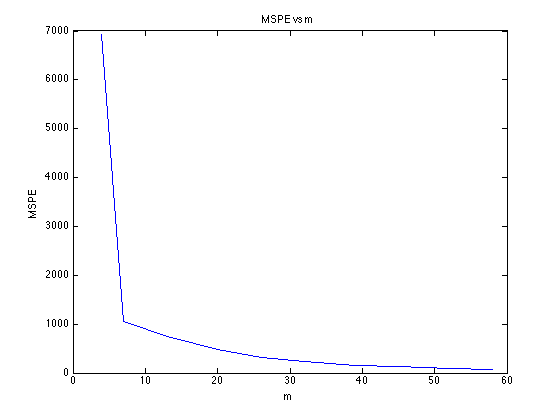
\includegraphics[width=3.5in]{hw5_11.png}
			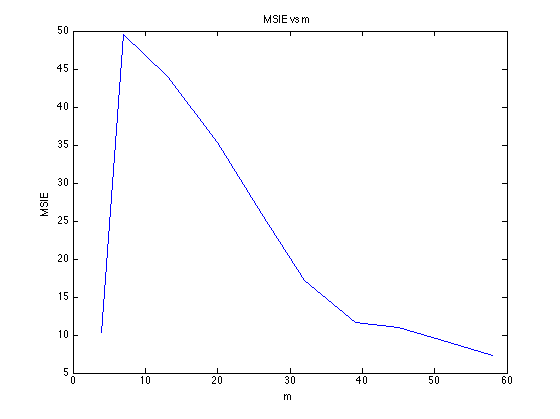
\includegraphics[width=3.5in]{hw5_12.png}
			\caption{Results for original experiment}
		\end{figure}
		
		\begin{figure}[h]
			\centering
			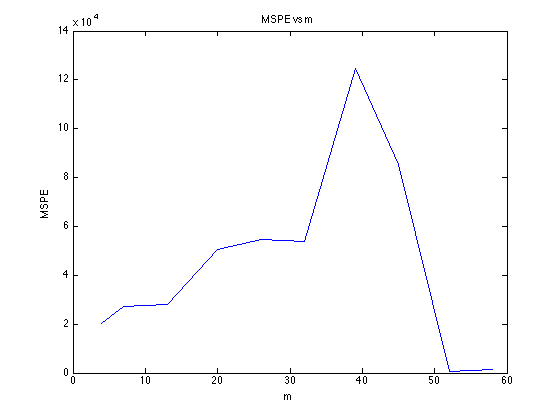
\includegraphics[width=3.5in]{hw5_2_11.png}
			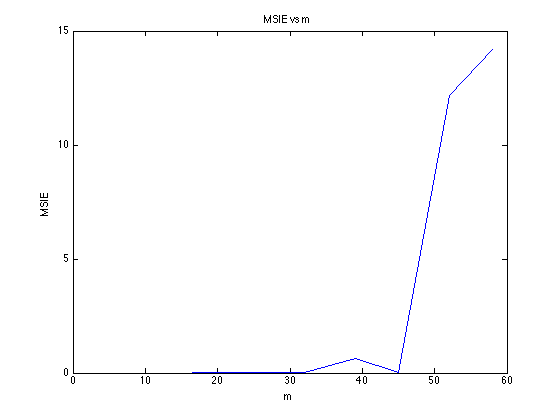
\includegraphics[width=3.5in]{hw5_2_12.png}
			\caption{Results for psuedo inverse experiment}
		\end{figure}
		
		\begin{figure}[h]
			\centering
			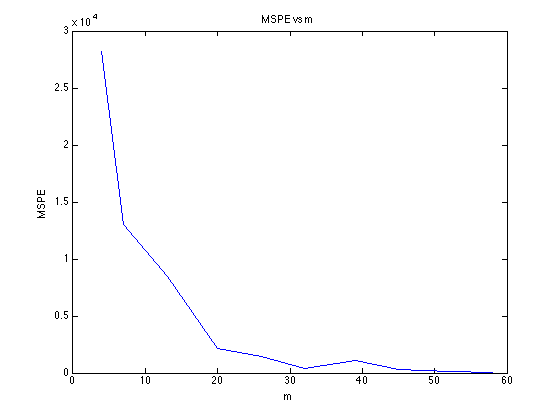
\includegraphics[width=3.5in]{hw5_3_11.png}
			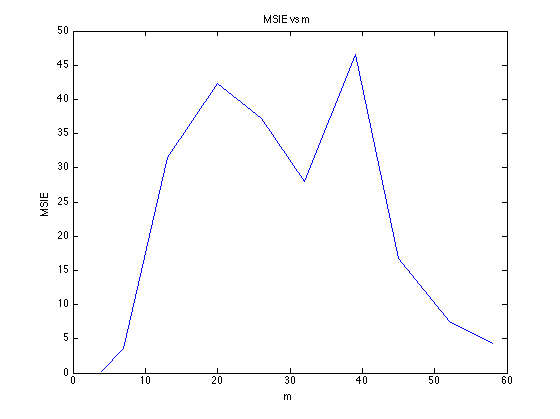
\includegraphics[width=3.5in]{hw5_3_12.png}
			\caption{Results for $\phi_m = $ random rows of $U^T$ experiment}
		\end{figure}
\end{itemize}

\end{enumerate}



\end{document}